\documentclass{article}

\usepackage[spanish]{babel}
\usepackage[numbers,sort&compress]{natbib}
\usepackage[T1]{fontenc}
\usepackage[ansinew]{inputenc}
\usepackage{graphicx}
\usepackage{url}
\usepackage{subcaption}
\usepackage{caption}
\usepackage{listings}
\usepackage{enumerate}
\usepackage{amsmath}
\usepackage{float}
\usepackage[numbers,sort&compress]{natbib}

\begin{document}
\title{\textbf{Algoritmo gen\'etico}}
\author{Anahi Elizabeth Llano}

\maketitle

\section{Objetivo}\label{obj}

En esta pr\'actica se analiza un modelo representativo del comportamiento de selecci\'on de variables que representa la gen\'etica. Se utiliza un m\'etodo de optimizaci\'on el cual es, el problema de la mochila, el cual determina cuales elementos son necesarios para obtener un resultado determinado ya que en este caso la mochila cuenta con un l\'imite de capacidad. Este algoritmo selecciona la combinaci\'on de funciones m\'as eficientes de tal manera que se pueda aceptar o no el que un elemento ingrese en la mochila.
La pr\'actica \cite{elisa} consiste en variar el problema de la mochila ya mencionado, creando tres escenarios diferentes para ello. En el primero los pesos y los valores generados son independientes, en el segundo se generan los pesos y se correlacionan los valores, y en el tercer escenario se generan los pesos y se correlacionan de manera inversa los valores, todo esto variando la selecci\'on de padres a manera de selecci\'on tipo ruleta, variando los tres casos a partir de qu\'e tama\~no de instancia el algoritmo gen\'etico es mejor que el algoritmo exacto en t\'erminos de valor total obtenido por segundo de ejecuci\'on y de esta manera determinar si la inclusi\'on de la selecci\'on de ruleta produce una mejora estad\'isticamente significativa.


\section{Metodolog\'{i}a}\label{met}

Se realiz\o una modificaci\'on en el \'ultimo c\'odigo mostrado en clase \citep{elisa}, de tal manera de generar las $3$ instancias:
Los pesos y los valores generados son independientes.
Se generan los pesos y se correlacionan los valores.
Se generan los pesos y se correlacionan de manera inversa los valores.
Una vez generados los puntos mencionados, se prosigui\'o a cambiar la selecci\'on de padres a que fueran tipo ruleta, buscando que cada padre posea una probabilidad de ser elegido que ser\'ia directamente proporcional a su valor de funci\'on objetivo y su factibilidad, de tal manera de cumplir con el objetivo de la tarea determinando para cada uno de los tres casos a partir de qu\'e tama\~no de instancia el algoritmo gen\'etico es mejor que el algoritmo exacto en t\'erminos de valor total obtenido por segundo de ejecuci\'on y si la inclusi\'on de la selecci\'on de ruleta produce una mejora estad\'isticamente significativa \citep{elisadisc}.


\section{Resultados y Discusi\'{o}n}\label{res}

 En la figura \ref{f1} se observa el efecto que tuvo el cambio de m\'etodo de selecci\'on, se muestra que con el m\'etodo de selecci\'on ruleta se muestran mejoras en comparaci\'on con el aleatorio, cuando la cantidad de objetos es menor, sin embargo, conforme aumentamos la cantidad de objetos, resulta ser mejor el aleatorio en comparaci\'on con el m\'etodo ruleta.

\begin{figure}[H]
       \centering
       \begin{subfigure}[b]{0.85\linewidth}
           \includegraphics[width=\linewidth]{P10r20.png}
           \caption{20 objetos}
           \label{fig:westminster_lateral}
        \end{subfigure}
        \begin{subfigure}[b]{0.85\linewidth}
            \includegraphics[width=\linewidth]{P10r40.png}
            \caption{40 objetos}
            \label{fig:westminster_aerea}
        \end{subfigure}
        \caption{Comparacion ruleta con diferentes objetos.}
        \label{f1}
\end{figure}

Tambi\'en fue modificado el c\'odigo \citep{ana} para evaluar la mejora con $3$ distintas instancias:
\begin{itemize} \item El peso y el valor de cada objeto se generan independientemente con una distribuci\'on exponencial. \item El peso de cada objeto se generan independientemente con una distribuci\'on exponencial y su valor es (positivamente) correlacionado con el peso, con un ruido normalmente distribuido de baja magnitud. \item El peso de cada objeto se generan independientemente con una distribuci\'on exponencial y su valor es inversamente correlacionado con el peso, con un ruido normalmente distribuido de baja magnitud.
\end{itemize}

Esto se evalu\'o en diferentes valores en $n$, es decir en la cantidad de objetos, y los resultados se muestran en el cuadro \ref{t1} , donde podemos comparar el valor \'optimo del mejor valor generado para diferentes $n$, $20$, $40$, $80$, $100$ y $120$, esto para cada una de las instancias mencionadas.

\begin{table} [H]
 \caption{Datos obtenidos con las 3 reglas a diferente n\'umero de objetos.}
 \label{t1}
 \begin{center}
 \begin{tabular}{rrrrrrr}
\texttt{Objetos} & \texttt{Mayor Valor} & \texttt{\'Optimo} &\texttt{Instancia} \\
20  & 1282.013322048552   & 1296.6201550491073  & 1  \\ 
20  & 4787.9432414394905 & 4787.943241439491    & 2\\ 
20  & 3604.9873301831326 & 3604.9873301831326  & 3  \\ 
40  &1434.0228352756253  &1441.3226000679583  & 1   \\ 
40  & 9501.850479218307   &9520.19704278877 & 2 \\ 
40  & 9209.251465178459   &9209.251465178457  & 3   \\ 
80  & 1686.7157670674028 & 1701.3226000679583 & 1 \\ 
80  & 18554.155582097403 & 19521.571770984312 & 2  \\ 
80  &18545.438991167717  &19301.725973425924  & 3  \\ 
100 & 1831.3226000679583&1831.3226000679585  & 1  \\ 
100 & 21648.405094569167&22468.387936264175  & 2   \\ 
100 & 21716.411383364262& 23146.710922689716  & 3 \\ 
120 & 1961.3226000679585& 1961.3226000679585  & 1  \\ 
120 &27430.592303774454 &29109.191853721157  & 2  \\ 
120 &24757.55728136999   &26928.537475636997 & 3  \\ 

\end{tabular}
\end{center}
\end{table}

De manera gr\'afica se observa en la figura \ref{f2} el comportamiento de las 3 diferentes instancias con $n=80$ 

\begin{figure}[H]
       \centering
       \begin{subfigure}[b]{0.8\linewidth}
           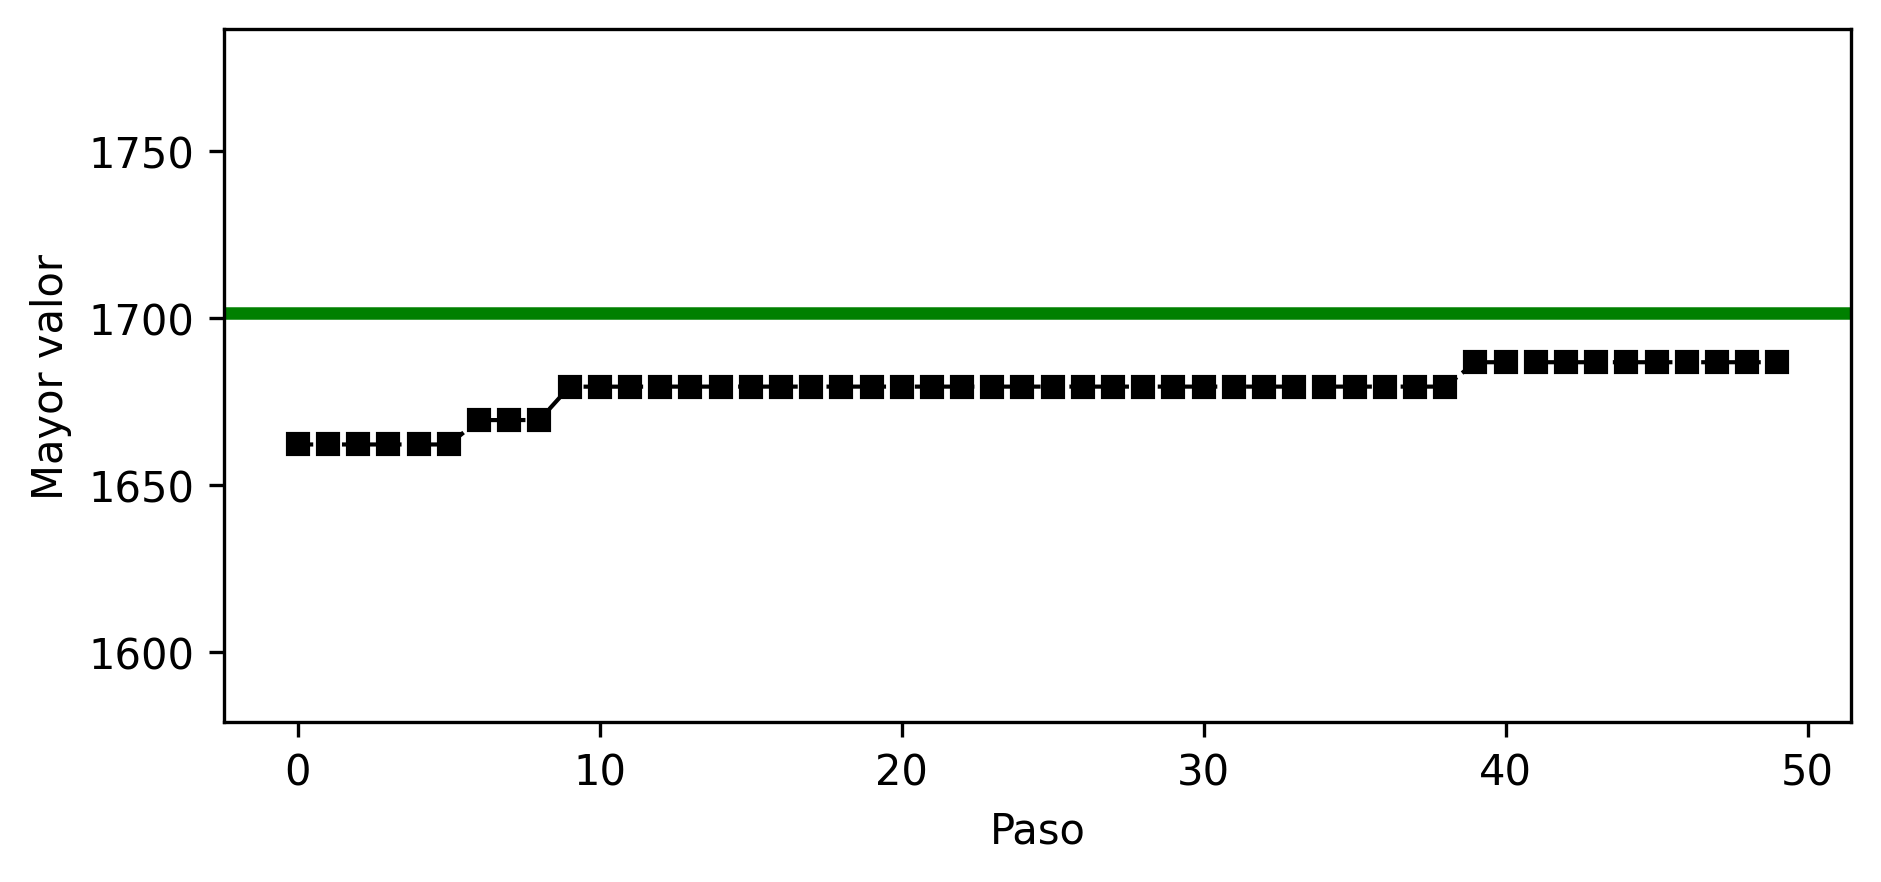
\includegraphics[width=\linewidth]{80i1.png}
           \caption{instancia $1$}
           \label{fig:westminster_lateral}
        \end{subfigure}
        \begin{subfigure}[b]{0.8\linewidth}
            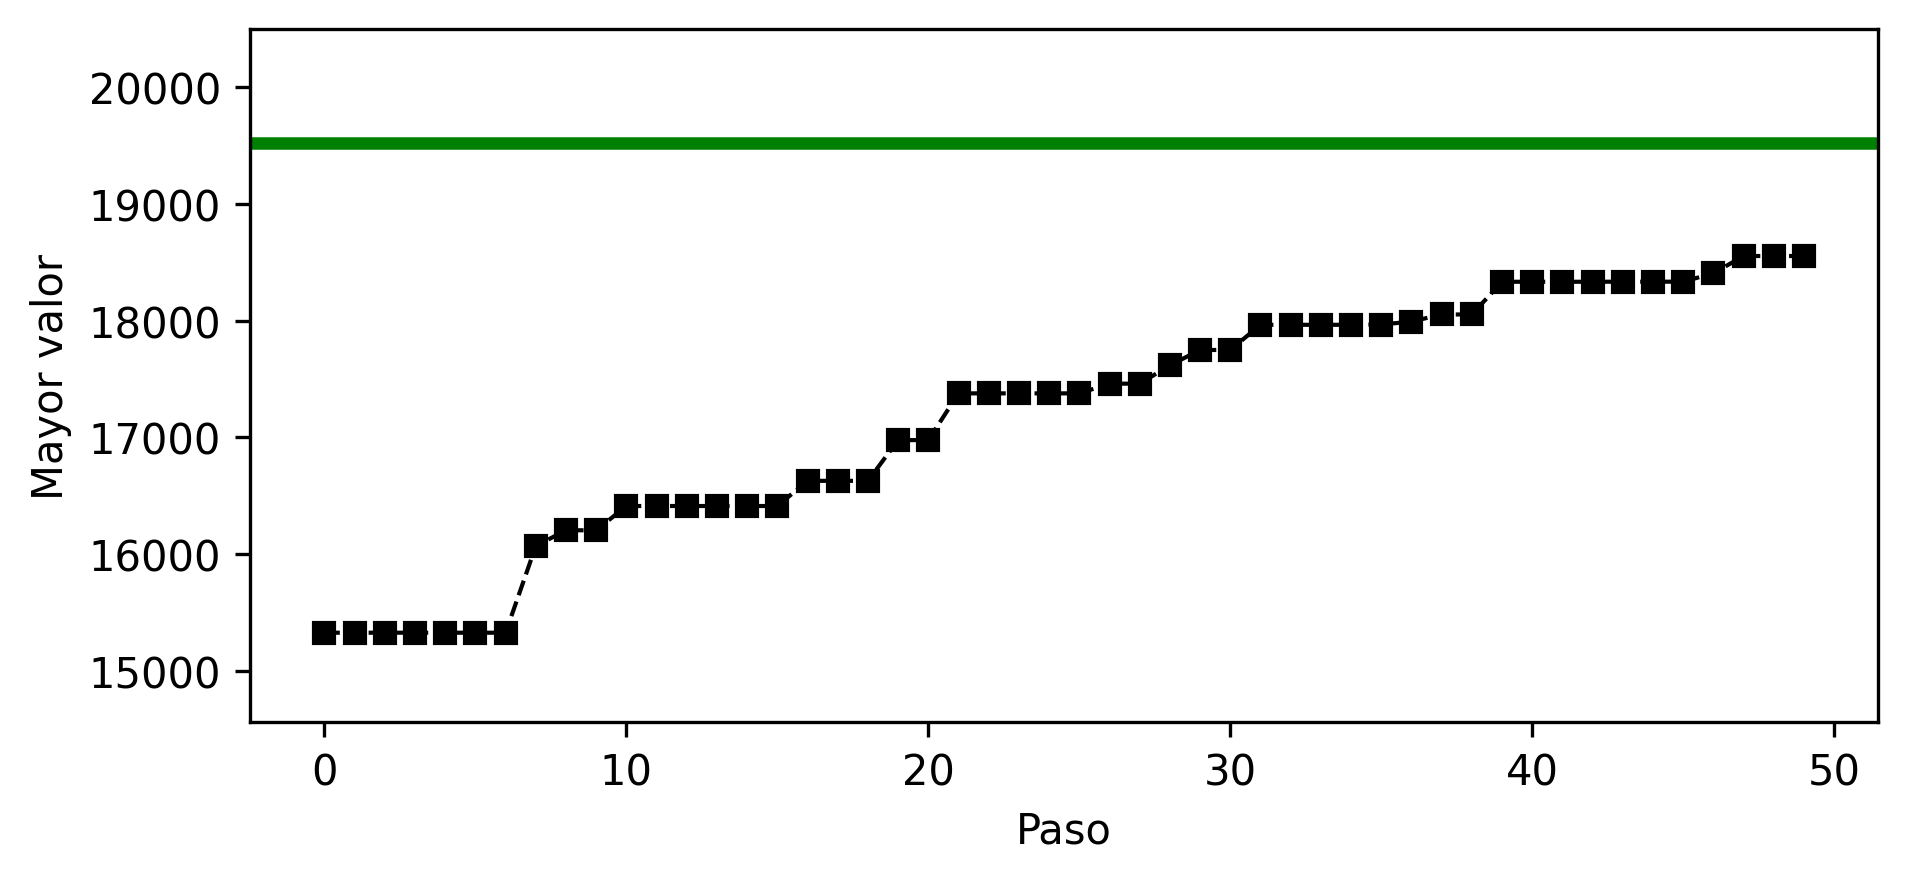
\includegraphics[width=\linewidth]{8012.png}
            \caption{instancia $2$}
            \label{fig:westminster_aerea}
        \end{subfigure}
        \begin{subfigure}[b]{0.8\linewidth}
           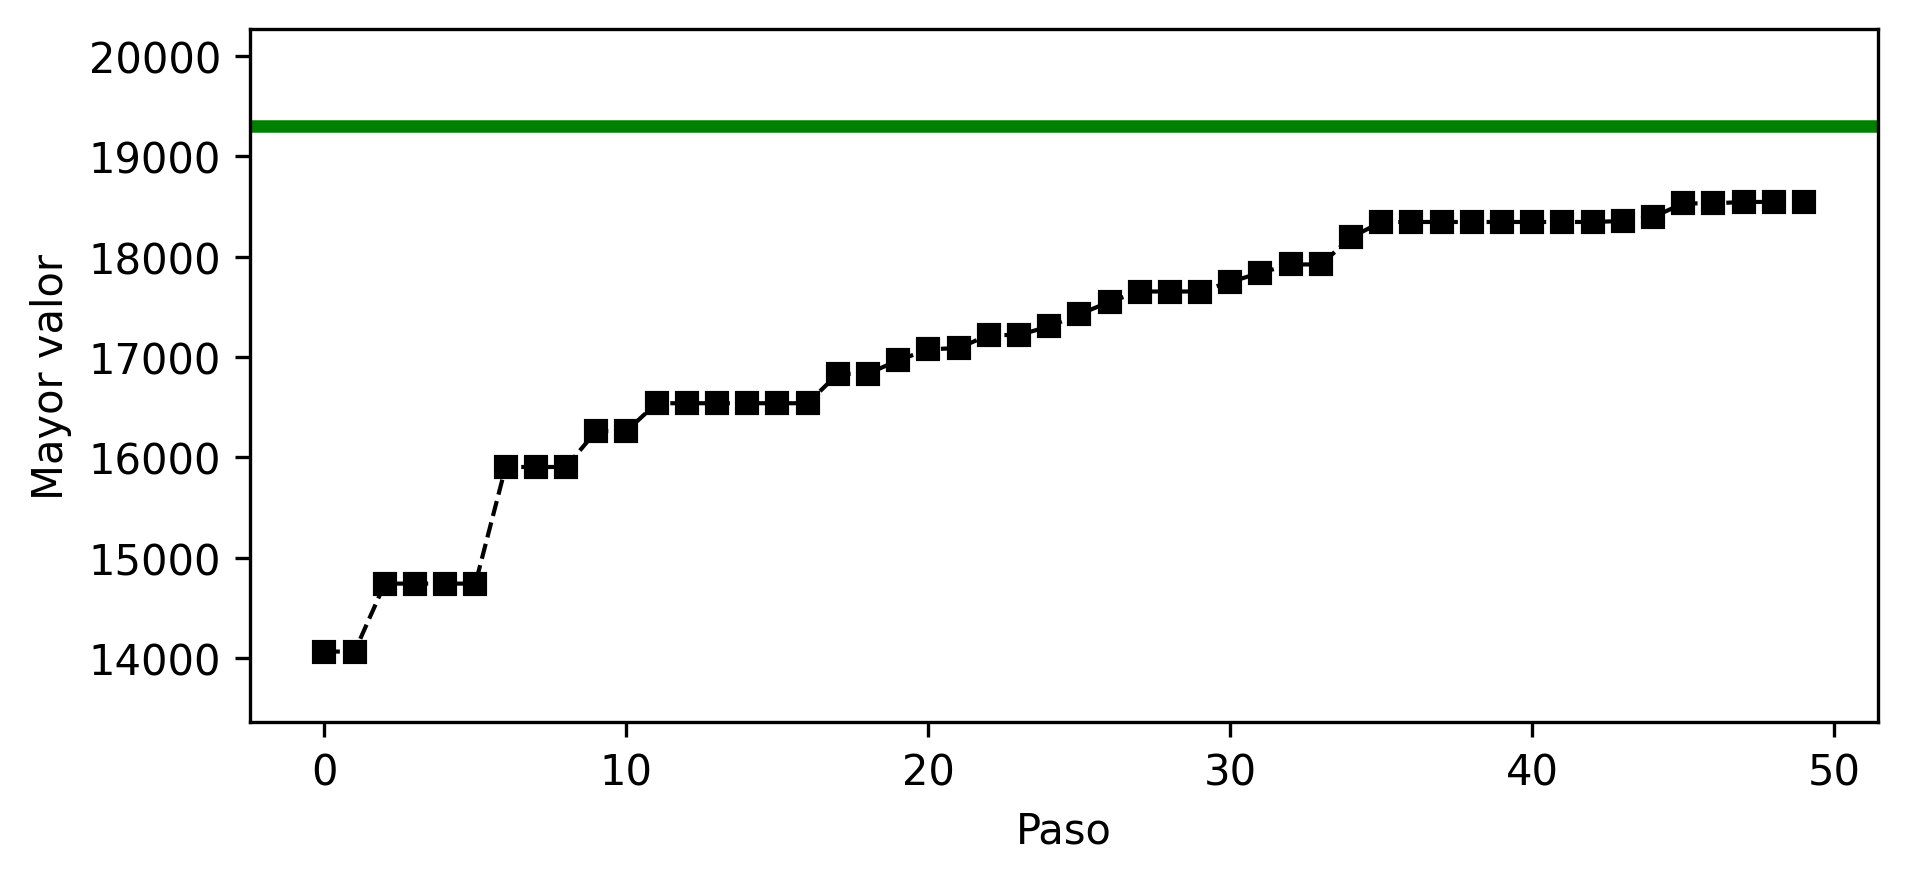
\includegraphics[width=\linewidth]{80i3.png}
           \caption{instancia $3$}
           \label{fig:westminster_aerea}
        \end{subfigure}
        \caption{Comparaci\'on de las $3$ instancias tomando $80$ objetos}
        \label{f2}
\end{figure}

De manera gr\'afica se observa en la figura \ref{f3} el comportamiento de las 3 diferentes instancias con $n=20$ 

\begin{figure}[H]
       \centering
       \begin{subfigure}[b]{0.8\linewidth}
           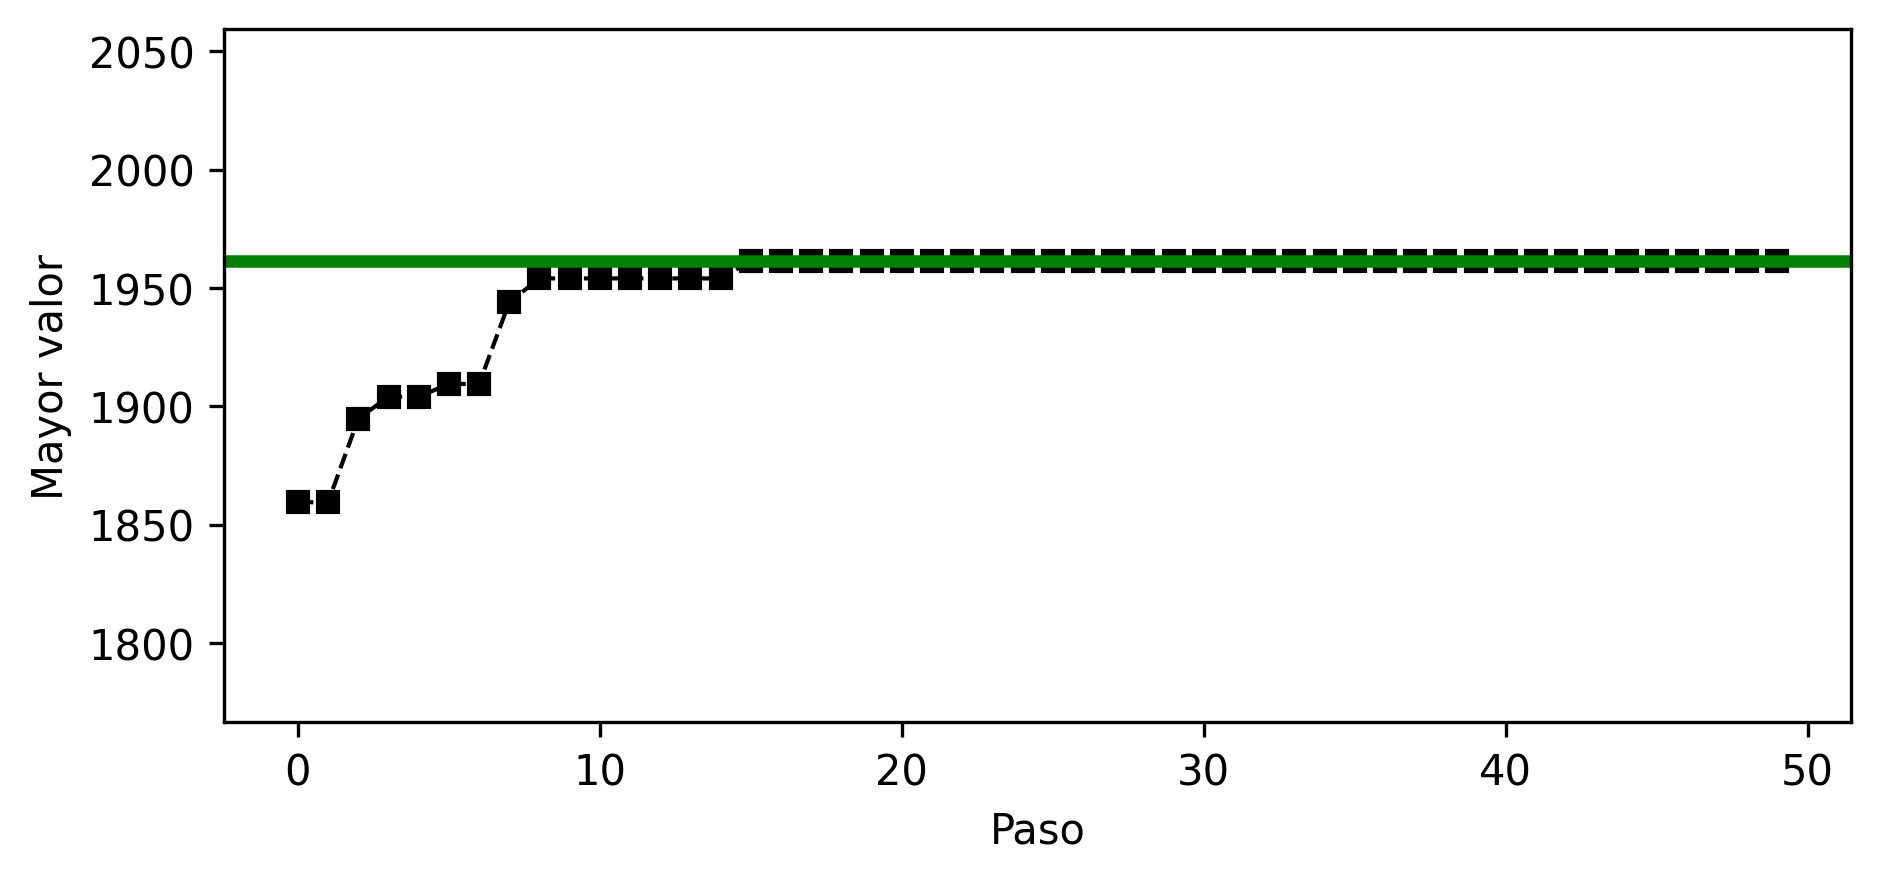
\includegraphics[width=\linewidth]{20i1.png}
           \caption{instancia $1$}
           \label{fig:westminster_lateral}
        \end{subfigure}
        \begin{subfigure}[b]{0.8\linewidth}
            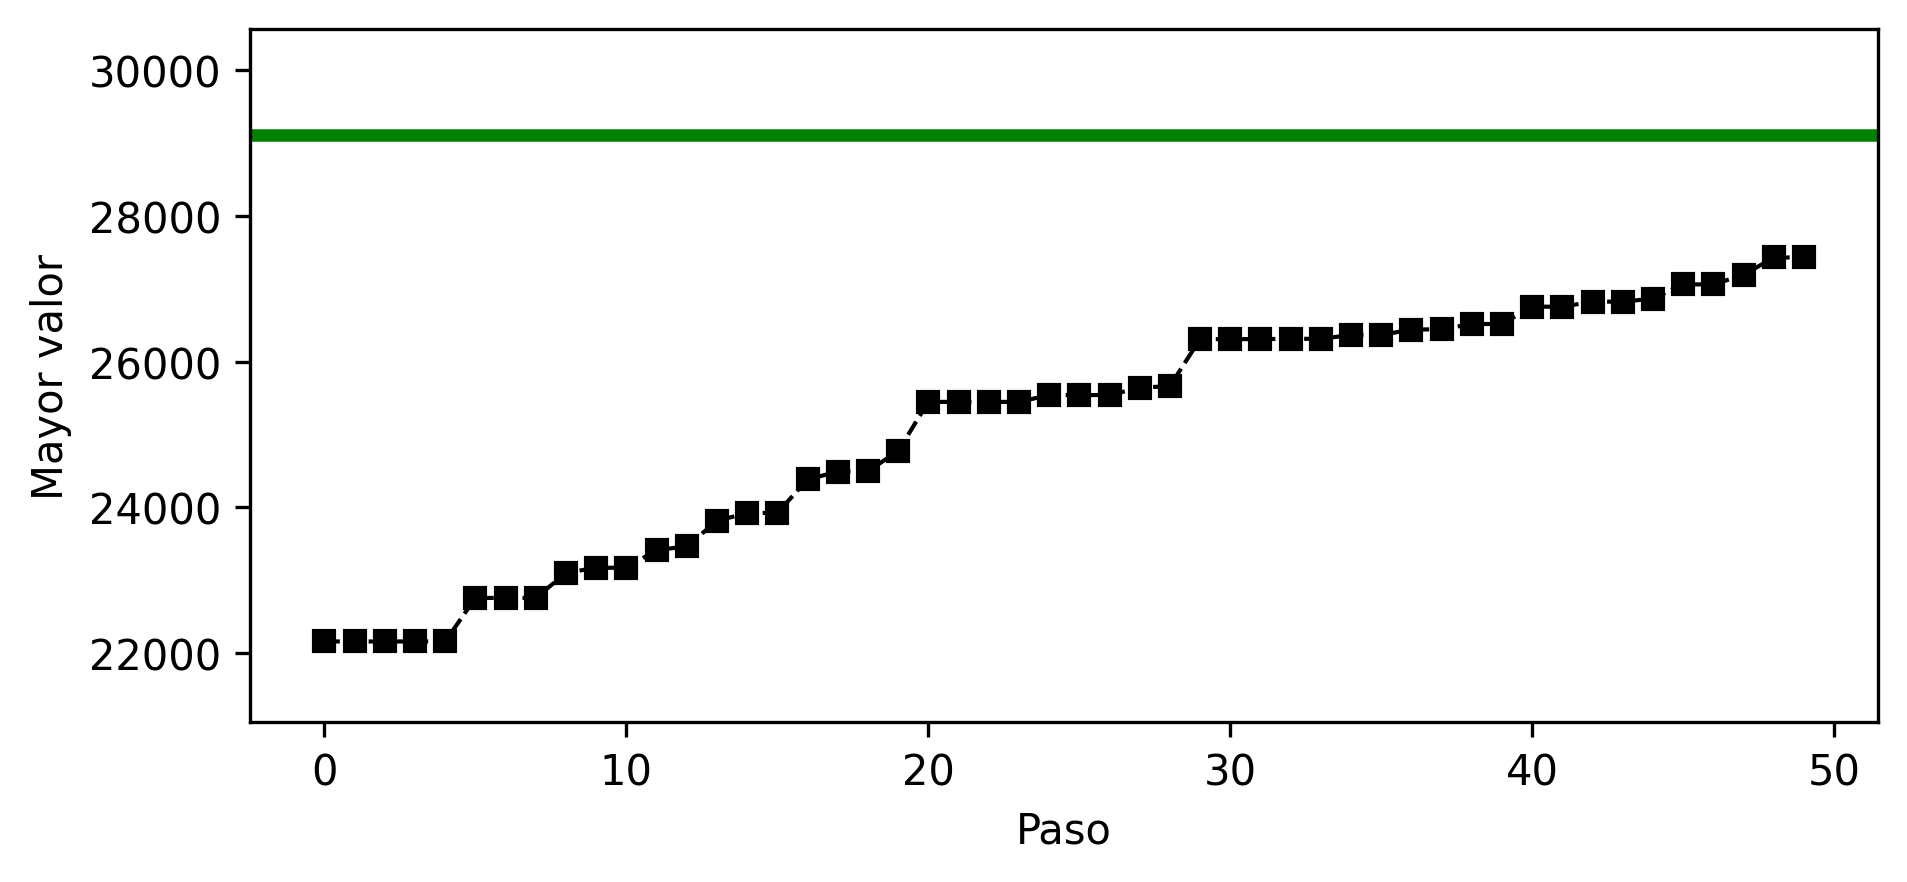
\includegraphics[width=\linewidth]{20i2.png}
            \caption{instancia $2$}
            \label{fig:westminster_aerea}
        \end{subfigure}
        \begin{subfigure}[b]{0.8\linewidth}
           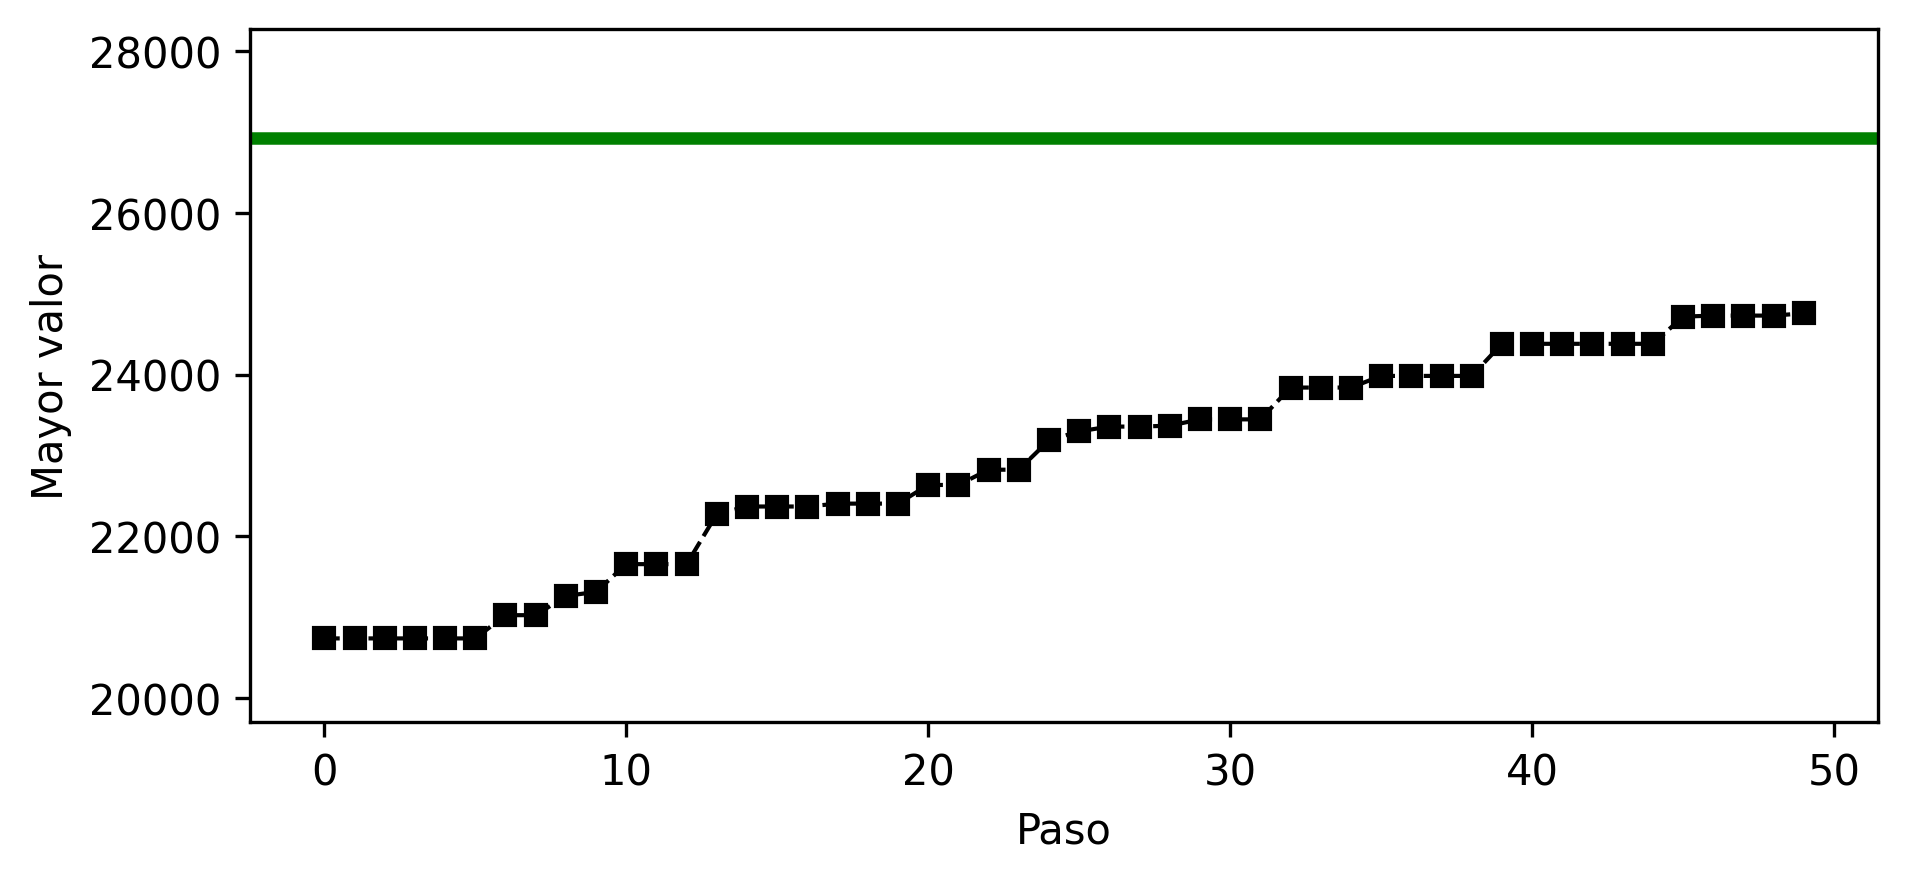
\includegraphics[width=\linewidth]{20i3.png}
           \caption{instancia $3$}
           \label{fig:westminster_aerea}
        \end{subfigure}
        \caption{Comparacion de las $3$ instancias tomando $20$ objetos}
        \label{f3}
\end{figure}
\section{Conclusi\'{o}n}\label{con}

Se muestra el impacto causado por el efecto utilizando un m\'etodo de selecci\'on de padres diferente, en este caso tipo ruleta, en donde se observ\'o que el m\'etodo logra acercarse a la soluci\'on \'optima en menos generaciones, sin embargo, pierde valor al avanzar a generaciones futuras en donde es alcanzado por el m\'etodo aleatorio. Adicionalmente se observa en las $3$ instancias generadas, que la mejor instancia en donde nos acerc\'abamos m\'as al valor \'optimo fue en la $1$ tanto para cuando tenemos $20$ como cuando tenemos $80$ objetos.

  \bibliography{P10}
  \bibliographystyle{plainnat}
\end{document}